\documentclass[12pt]{extreport}
\usepackage[T2A]{fontenc}
\usepackage[utf8]{inputenc}        % Кодировка входного документа;
                                    % при необходимости, вместо cp1251
                                    % можно указать cp866 (Alt-кодировка
                                    % DOS) или koi8-r.

\usepackage[english,russian]{babel} % Включение русификации, русских и
                                    % английских стилей и переносов
%%\usepackage{a4}
%%\usepackage{moreverb}
\usepackage{amsmath,amsfonts,amsthm,amssymb,amsbsy,amstext,amscd,amsxtra,multicol}
\usepackage{indentfirst}
\usepackage{verbatim}
\usepackage{tikz} %Рисование автоматов
\usetikzlibrary{automata,positioning}
%\usepackage{multicol} %Несколько колонок
\usepackage{graphicx}
\usepackage[colorlinks,urlcolor=blue]{hyperref}
\usepackage[stable]{footmisc}

%% \voffset-5mm
%% \def\baselinestretch{1.44}
\renewcommand{\theequation}{\arabic{equation}}
\def\hm#1{#1\nobreak\discretionary{}{\hbox{$#1$}}{}}
\newtheorem{Lemma}{Лемма}
\theoremstyle{definiton}
\newtheorem{Remark}{Замечание}
%%\newtheorem{Def}{Определение}
\newtheorem{Claim}{Утверждение}
\newtheorem{Cor}{Следствие}
\newtheorem{Theorem}{Теорема}
\theoremstyle{definition}
\newtheorem{Example}{Пример}
\newtheorem*{known}{Теорема}
\def\proofname{Доказательство}
\theoremstyle{definition}
\newtheorem{Def}{Определение}

%% \newenvironment{Example} % имя окружения
%% {\par\noindent{\bf Пример.}} % команды для \begin
%% {\hfill$\scriptstyle\qed$} % команды для \end






%\date{22 июня 2011 г.}
\let\leq\leqslant
\let\geq\geqslant
\def\MT{\mathrm{MT}}
%Обозначения ``ажуром''
\def\BB{\mathbb B}
\def\CC{\mathbb C}
\def\RR{\mathbb R}
\def\SS{\mathbb S}
\def\ZZ{\mathbb Z}
\def\NN{\mathbb N}
\def\FF{\mathbb F}
%греческие буквы
\let\epsilon\varepsilon
\let\es\varnothing
\let\eps\varepsilon
\let\al\alpha
\let\sg\sigma
\let\ga\gamma
\let\ph\varphi
\let\om\omega
\let\ld\lambda
\let\Ld\Lambda
\let\vk\varkappa
\let\Om\Omega
\def\abstractname{}

\def\R{{\cal R}}
\def\A{{\cal A}}
\def\B{{\cal B}}
\def\C{{\cal C}}
\def\D{{\cal D}}

%классы сложности
\def\REG{{\mathsf{REG}}}
\def\CFL{{\mathsf{CFL}}}


%%%%%%%%%%%%%%%%%%%%%%%%%%%%%%% Problems macros  %%%%%%%%%%%%%%%%%%%%%%%%%%%%%%%


%%%%%%%%%%%%%%%%%%%%%%%% Enumerations %%%%%%%%%%%%%%%%%%%%%%%%

\newcommand{\Rnum}[1]{\expandafter{\romannumeral #1\relax}}
\newcommand{\RNum}[1]{\uppercase\expandafter{\romannumeral #1\relax}}

%%%%%%%%%%%%%%%%%%%%% EOF Enumerations %%%%%%%%%%%%%%%%%%%%%

\usepackage{xparse}
\usepackage{ifthen}
\usepackage{bm} %%% bf in math mode
\usepackage{color}
%\usepackage[usenames,dvipsnames]{xcolor}

\definecolor{Gray555}{HTML}{555555}
\definecolor{Gray444}{HTML}{444444}
\definecolor{Gray333}{HTML}{333333}


\newcounter{problem}
\newcounter{uproblem}
\newcounter{subproblem}
\newcounter{prvar}

\def\beforPRskip{
	\bigskip
	%\vspace*{2ex}
}

\def\PRSUBskip{
	\medskip
}


\def\pr{\beforPRskip\noindent\stepcounter{problem}{\bf \theproblem .\;}\setcounter{subproblem}{0}}
\def\pru{\beforPRskip\noindent\stepcounter{problem}{\bf $\mathbf{\theproblem}^\circ$\!\!.\;}\setcounter{subproblem}{0}}
\def\prstar{\beforPRskip\noindent\stepcounter{problem}{\bf $\mathbf{\theproblem}^*$\negthickspace.}\setcounter{subproblem}{0}\;}
\def\prpfrom[#1]{\beforPRskip\noindent\stepcounter{problem}{\bf Задача \theproblem~(№#1 из задания).  }\setcounter{subproblem}{0} }
\def\prp{\beforPRskip\noindent\stepcounter{problem}{\bf Задача \theproblem .  }\setcounter{subproblem}{0} }

\def\prpvar{\beforPRskip\noindent\stepcounter{problem}\setcounter{prvar}{1}{\bf Задача \theproblem \;$\langle${\rm\Rnum{\theprvar}}$\rangle$.}\setcounter{subproblem}{0}\;}
\def\prpv{\beforPRskip\noindent\stepcounter{prvar}{\bf Задача \theproblem \,$\bm\langle$\bracketspace{{\rm\Rnum{\theprvar}}}$\bm\rangle$.  }\setcounter{subproblem}{0} }
\def\prv{\beforPRskip\noindent\stepcounter{prvar}{\bf \theproblem\,$\bm\langle$\bracketspace{{\rm\Rnum{\theprvar}}}$\bm\rangle$}.\setcounter{subproblem}{0} }

\def\prpstar{\beforPRskip\noindent\stepcounter{problem}{\bf Задача $\bf\theproblem^*$\negthickspace.  }\setcounter{subproblem}{0} }
\def\prdag{\beforPRskip\noindent\stepcounter{problem}{\bf Задача $\theproblem^{^\dagger}$\negthickspace\,.  }\setcounter{subproblem}{0} }
\def\upr{\beforPRskip\noindent\stepcounter{uproblem}{\bf Упражнение \theuproblem .  }\setcounter{subproblem}{0} }
%\def\prp{\vspace{5pt}\stepcounter{problem}{\bf Задача \theproblem .  } }
%\def\prs{\vspace{5pt}\stepcounter{problem}{\bf \theproblem .*   }
\def\prsub{\PRSUBskip\noindent\stepcounter{subproblem}{\sf \thesubproblem .} }
\def\prsubr{\PRSUBskip\noindent\stepcounter{subproblem}{\bf \asbuk{subproblem})}\;}
\def\prsubstar{\PRSUBskip\noindent\stepcounter{subproblem}{\rm $\thesubproblem^*$\negthickspace.  } }
\def\prsubrstar{\PRSUBskip\noindent\stepcounter{subproblem}{$\text{\bf \asbuk{subproblem}}^*\mathbf{)}$}\;}

\newcommand{\bracketspace}[1]{\phantom{(}\!\!{#1}\!\!\phantom{)}}

\DeclareDocumentCommand{\Prpvar}{ O{null} O{} }{
	\beforPRskip\noindent\stepcounter{problem}\setcounter{prvar}{1}{\bf Задача \theproblem
% 	\ifthenelse{\equal{#1}{null}}{  }{ {\sf $\bm\langle$\bracketspace{#1}$\bm\rangle$}}
%	~\!\!(\bracketspace{{\rm\Rnum{\theprvar}}}).  }\setcounter{subproblem}{0}
%	\;(\bracketspace{{\rm\Rnum{\theprvar}}})}\setcounter{subproblem}{0}
%
	\,{\sf $\bm\langle$\bracketspace{{\rm\Rnum{\theprvar}}}$\bm\rangle$}
	~\!\!\! \ifthenelse{\equal{#1}{null}}{\!}{{\sf(\bracketspace{#1})}}}.

}
%\DeclareDocumentCommand{\Prpvar}{ O{level} O{meta} m }{\prpvar}


\DeclareDocumentCommand{\Prp}{ O{null} O{null} }{\setcounter{subproblem}{0}
	\beforPRskip\noindent\stepcounter{problem}\setcounter{prvar}{0}{\bf Задача \theproblem
	~\!\!\! \ifthenelse{\equal{#1}{null}}{\!}{{\sf(\bracketspace{#1})}}
	 \ifthenelse{\equal{#2}{null}}{\!\!}{{\sf [\color{Gray444}\,\bracketspace{{\fontfamily{afd}\selectfont#2}}\,]}}}.}

\DeclareDocumentCommand{\Pr}{ O{null} O{null} }{\setcounter{subproblem}{0}
	\beforPRskip\noindent\stepcounter{problem}\setcounter{prvar}{0}{\bf\theproblem
	~\!\!\! \ifthenelse{\equal{#1}{null}}{\!\!}{{\sf(\bracketspace{#1})}}
	 \ifthenelse{\equal{#2}{null}}{\!\!}{{\sf [\color{Gray444}\,\bracketspace{{\fontfamily{afd}\selectfont#2}}\,]}}}.}

%\DeclareDocumentCommand{\Prp}{ O{level} O{meta} }

\DeclareDocumentCommand{\Prps}{ O{null} O{null} }{\setcounter{subproblem}{0}
	\beforPRskip\noindent\stepcounter{problem}\setcounter{prvar}{0}{\bf Задача $\bm\theproblem^* $
	~\!\!\! \ifthenelse{\equal{#1}{null}}{\!}{{\sf(\bracketspace{#1})}}
	 \ifthenelse{\equal{#2}{null}}{\!\!}{{\sf [\color{Gray444}\,\bracketspace{{\fontfamily{afd}\selectfont#2}}\,]}}}.
}

\DeclareDocumentCommand{\Prpd}{ O{null} O{null} }{\setcounter{subproblem}{0}
	\beforPRskip\noindent\stepcounter{problem}\setcounter{prvar}{0}{\bf Задача $\bm\theproblem^\dagger$
	~\!\!\! \ifthenelse{\equal{#1}{null}}{\!}{{\sf(\bracketspace{#1})}}
	 \ifthenelse{\equal{#2}{null}}{\!\!}{{\sf [\color{Gray444}\,\bracketspace{{\fontfamily{afd}\selectfont#2}}\,]}}}.
}


\def\prend{
	\bigskip
%	\bigskip
}




%%%%%%%%%%%%%%%%%%%%%%%%%%%%%%% EOF Problems macros  %%%%%%%%%%%%%%%%%%%%%%%%%%%%%%%



%\usepackage{erewhon}
%\usepackage{heuristica}
%\usepackage{gentium}

\usepackage[portrait, top=3cm, bottom=1.5cm, left=3cm, right=2cm]{geometry}

\usepackage{fancyhdr}
\pagestyle{fancy}
\renewcommand{\headrulewidth}{0pt}
\lhead{\fontfamily{fca}\selectfont {ФПМИ. Основные алгоритмы 2022} }
%\lhead{ \bf  {ТРЯП. } Семинар 1 }
%\chead{\fontfamily{fca}\selectfont {Вариант 1}}
\rhead{\fontfamily{fca}\selectfont Домашнее задание 10. Павлов М.А.}
%\rhead{\small 01.09.2016}
\cfoot{}

\usepackage{titlesec}
\titleformat{\section}[block]{\Large\bfseries\filcenter {\setcounter{problem}{0}}  }{}{1em}{}


%%%%%%%%%%%%%%%%%%%%%%%%%%%%%%%%%%%%%%%%%%%%%%%%%%%% Обозначения и операции %%%%%%%%%%%%%%%%%%%%%%%%%%%%%%%%%%%%%%%%%%%%%%%%%%%% 
                                                                    
\newcommand{\divisible}{\mathop{\raisebox{-2pt}{\vdots}}}           
\let\Om\Omega


%%%%%%%%%%%%%%%%%%%%%%%%%%%%%%%%%%%%%%%% Shen Macroses %%%%%%%%%%%%%%%%%%%%%%%%%%%%%%%%%%%%%%%%
\newcommand{\w}[1]{{\hbox{\texttt{#1}}}}

\newcommand{\Prob}{\mathop{\mathrm{P}}}
\newcommand{\Ex}{\mathop{\mathrm{E}}}

\usepackage[linesnumbered]{algorithm2e}   

\begin{document}
	


\pr В графе может быть несколько кратчайших путей между какими-то вершинами\ldots

	Поскольку вес каждого ребра равен 1, то мы спокойно можем свести задачу к поиску всех минимальных подграфов-путей из $s$ в $t$.

	На семинаре было разобрано, что вполне оптимальным для решения данной задачи является BFS, который работает за линейное время $O(|V| + |E|)$.

	Как мы будем его использовать?

	1) Раскрашиваем все соединяющие вершины на расстоянии 1 от начала ребра в серый цвет.

	2) Раскрашиваем в серый цвет все вершины, в которые мы пришли.

	3) Продолжаем те же действия, но уже на i-той итерации раскрашиваем все ребра, соединяющие вершины на расстоянии $i$. Однако, если вершина, в которую мы хотим пойти, уже раскрашена, то ребро не трогаем.

	4) Как только на какой-то итерации мы дошли до вершины $t$, заканчиваем поиск и идем обратно по закрашенным ребрам. Все пройденные вершины при этом закрашиваем в красный цвет.

	Красные вершины и будут искомыми.

	Оценка по времени: совпадает с BFS, то есть $\theta(|V| + |E|)$.

	Корректность: действительно, если мы на $k$-той итерации добрались до конечной вершины, то никаких путей длиннее и короче $k$ мы не находили (поскольку для длинных путей требовалось бы больше итераций).
	Значит, количство вершин на простых путях от $t$ в $s$ будет искомым числом, поскольку все эти вершины лежат на одном из кратчайших путей.

\medskip

%\upr Приведите пример взвешенного ориентированного графа, на котором алгоритм Дейкстры \prsubr находит кратчайшие пути неправильно; \prsubr находит кратчайшие пути правильно. Продемонстрируйте работу алгоритма на первом примере.

%\medskip\noindent\textsl{Упражнения не входят в обязательную часть домашнего задания.}
%\prend

\pr Рассмотрим следующую модификацию алгоритма Дейкстры\ldots

\prsub Докажите корректность модифицированного алгоритма. 

	По сути грубо говоря этот алгоритм отличается от оригинального тем, что при выборе минимальной вершины мы не обращаем внимания на те, расстояние до которыз равно бесконечности.

	В оригинальном алгоритме эти вершины могли стать минимальными только в том случае, если не осталось достижимых вершин, то есть поиск прошел неудачно. Значит, единственное отличие -- в данной модификации мы не забрасываем в очередь ненужные значения, что на корректность алгоритма не влияет.

	Следовательно, модификация имеет ту же корректность, что и сам оригинальный алгоритм, то есть модификация корректна.

\prsub Докажите, что модифицированный алгоритм работает корректно даже в случае наличия рёбер отрицательного веса, но при отсутсвии цикла отрицательного веса. Оцените время работы алгоритма на графах такого вида и сравните его со временем работы алгоритма Беллмана-Форда.

	В момент, когда в нашей очереди останутся только вершины, которые там уже лежали, суммарный вес путей будет лишь убывать. Поскольку отрицательных циклов в графе нет по условию,
	то вечно он убывать не сможет и когда-нибудь обязательно остановится. Значит, он выполнит свою задачу, несмотря на ребра отрицательного веса.

	Заметим, что асимптотически после модификации сложность алгоритма не изменилась. Следовательно, модифицированный алгоритм Дейкстры, как и оригинальный, работает быстрее алгоритма Беллмана-Форда.

\prsub Модифицируйте алгоритм так, чтобы он выдавал ошибку на графах с циклами отрицательного веса.

	Когда все элементы будут в очереди, запустим очередной цикл заново. Если суммарный вес путей уменьшится -- выдаем ошибку, поскольку данный факт будет свидетельствовать о наличии в графе отрицательного цикла.

\pr Профессор О. П. Рометчивый \ldots

	К сожалению, профессор слегка поспешил с предположением корректности данного алгоритма. Контрпример моментально возникает в голове у любого человека, посещающего лекции Александра Александровича.

\begin{wrapfigure}
	\centering
	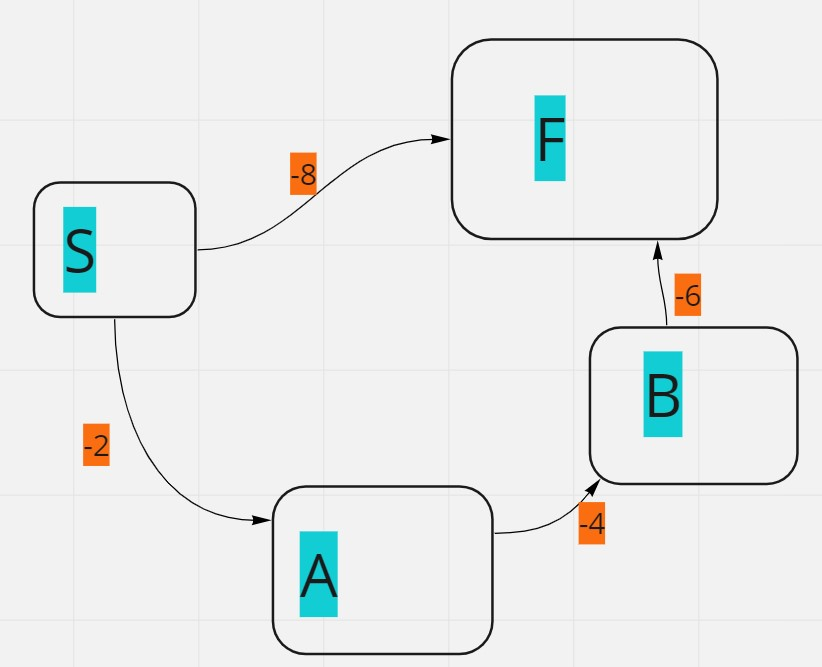
\includegraphics[scale=0.6]{1}
	\caption{Контрпример}
\end{wrapfigure}

	На изображении мы видим, что если добавить, к примеру, 9, то по алгоритму Дейкстры кратчайший путь от S к F будет SF, хотя на самом деле он равен SABF.

\pr Алгоритм поиска кратчайших расстояний от данной вершины $s$ до всех остальных в графе \ldots

	По сути здесь нам никто не запрещает использовать алгоритм поиска в ширину. По времени он как раз работает за нужное нам $O(|V| + |E|)$. По сути получается, что мы на каждой $i$-той итерации находим вершины, находящиеся на расстоянии $i$ от старта.

	Однако, наш алгоритм будет все же немного отличаться, а именно в случае с весом ребра $0$ мы стягиваем две эти вершины и представляем их как одну (суммируя ребра).

	Корректность следует их корректности BFS.


\pr Алгоритм, который находит для данной вершины вершину, \textbf{от которой} она удалена на максимальное расстояние \ldots.

	По сути здесь мы можем использовать алгоритм Беллмана-Форда, но в нем везде поменять знаки на противоположные. То есть при каждом сравнении мы выбираем не наименьшее значение, а наибольшее.

	Корректность очевидно и следует из корректности алгоритма Беллмана-Форда (по сути мы просто поменяли знаки местами, так что корректность не нарушилась).

	Время работы тоже совпадает с временем работы алгоритма Беллмана-Форда, то есть равно $\theta(|V||E|)$.


\end{document}
  